\subsection{Oracle}
\subsubsection{Oracle Architektur}


\begin{figure}[ht]
  \centering
  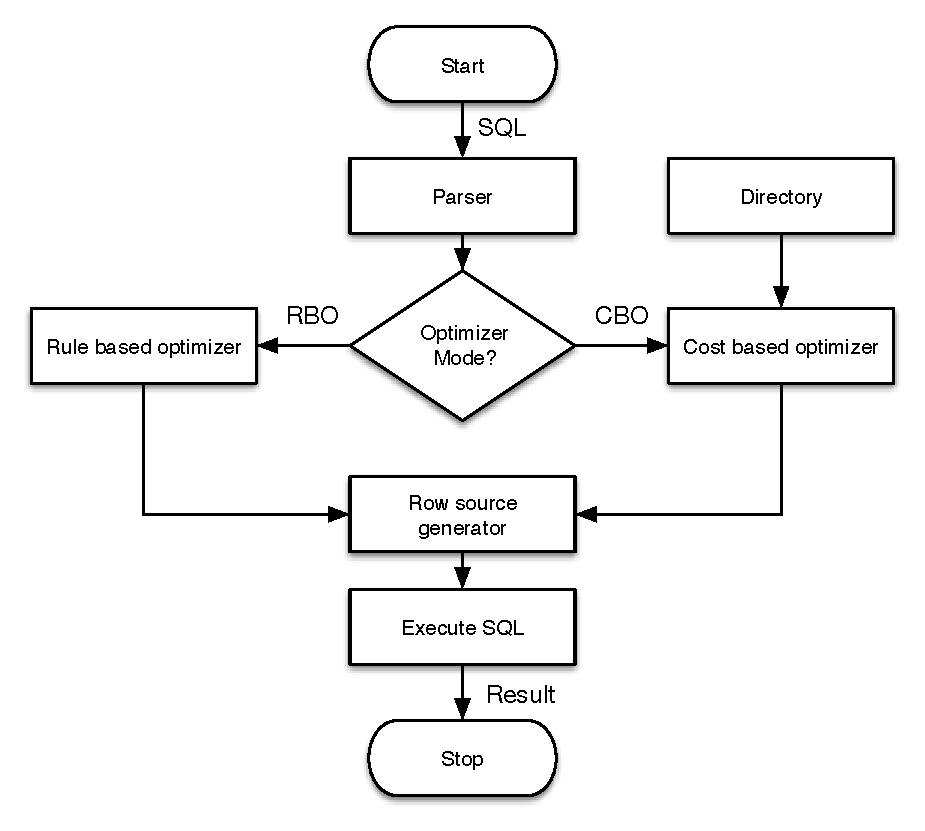
\includegraphics[width=\textwidth]{02_Related_Work/Oracle.pdf}
  \caption{Oracle Architecture \cite{Oracle2004Basics}}
  \label{OracleArchitecture}
\end{figure}


Die Oracle Architektur zur Verarbeitung von Anfragen \cite{Oracle2004Basics}  (vgl. Abb. \ref{OracleArchitecture})  beginnt wie die meisten Systeme mit einer SQL Anfrage, die von einem Parser in eine Interne Repräsentation gebracht wird. Der Parser übernimmt dabei zwei Funktionen. Auf der einen Seite die syntaktische Analyse. Es wird geprüft, ob die SQL Anfrage die korrekte Syntax besitzt. Auf der anderen Seite eine semantische Analyse. Diese prüft beispielsweise ob Datenbank Objekte und Objekt-Attribute  korrekt referenziert werden. 

Ein wesentlicher Unterschied war bis zu Version 11g der Oracle Datenbank,  die Verwendung von \ac{RBO} und \ac{CBO}. Je nach Anfrage konnte durch den \ac{DBI} entschieden werden, ob \ac{RBO} bzw. \ac{CBO} zum Einsatz kommt. Mit Version 11g ist diese Möglichkeit weggefallen \cite{dba_oracle2015}. 

Der Anfrageoptimierer führt bei der Verarbeitung die drei folgenden Schritte aus:

\begin{itemize}
\item Eine Menge potenzieller Pläne wird basierend der SQL Anfrage selbst und aufgrund von Hinweisen, die durch den Nutzer eingegeben werden, generiert.

\item Der Optimierer schätzt die Kosten für jeden Plan basierend auf Kosteninformationen über die Anfrage und Storage Charakteristiken der Tabellen, Indexe und Partitionen, auf die durch ein Statement zugegriffen werden kann.

Die Kostenschätzung für den Zugriff auf entsprechende Datensätze und die Reihenfolge der Joins wird nach ihrem Verbrauch von Ressourcen wie I/O, CPU und Arbeitsspeicher geschätzt.

\item Der Optimierer vergleicht die Kosten der Pläne und wählt den kostengünstigsten Plan aus.
\end{itemize}

Das Ergebnis des Optimierers ist ein Plan, der zum Ausführen der Anfrage geeignet ist und als kosten-optimal eingeschätzt wird.


\subsubsection{Unterschiedliche Optimierungsansätze}



Bei Oracle ist es möglich zwischen zwei Optimierungsansätzen zu wählen. Der Nutzer kann entscheiden, ob er möglichst schnell das gesamte Resultat der Anfrage benötigt oder ob das erste Resultat möglichst schnell zurückgegeben werden soll. Bei der Optimierung auf alle Resultate geht es darum den Plan zu finden, der mit dem geringsten Ressourceneinsatz alle Zeilen einer Abfrage zurückgibt. Die Optimierung des Durchsatzes geschieht insbesondere durch die Verwendung von Full-Table-Scans anstatt von Index-Scans und der Verwendung von Sort-Merge-Joins anstatt von nested loop-joins. Wenn es hingegen wichtig ist, dass schnell das erste Ergebnis zurückgegeben wird, also die Antwortzeit minimiert werden soll, werden Index-Scans und nested-loop-joins eingesetzt.

Welcher Ansatz zur Suche nach dem optimalen Plan verwendet wird, kann durch den Nutzer festgelegt werden. Für Anwendungen wie Reports sind alle Zeilen einer Datenmenge wichtig. Hier empfiehlt es sich den Durchsatz als Maßstab der Optimierung zu wählen. Bei dynamischeren, interaktiven Anwendungen ist es nicht immer notwendig, dass sofort auf alle Daten zugegriffen werden muss, daher ist eine Optimierung der Antwortzeit angebracht.


\subsubsection{Kostenschätzung in Oracle}
Die Kostenschätzung von Oracle basiert auf drei Komponenten: Selektivität, Kardinalität und Kosten. Ziel der Kostenschätzung ist es, anhand der Kosten den günstigsten Plan auszuwählen. Dabei wird das Ziel der Optimierung nicht aus den Augen gelassen.

Die Selektivität bezeichnet das Verhältnis von Datensätzen, die vor Anwendung von Prädikaten vorhanden sind und Datensätzen, die nach der Anwendung noch weiterverarbeitet werden. Beispielsweise haben Prädikate, die eine Datenmenge nicht einschränken die Selektivität von 1.0. Werden jedoch durch ein Prädikat alle Datensätze ausgeschlossen, ergibt sich eine Selektivität von 0.0. Bei Joins zwischen zwei Datenmengen schränkt das Join-Prädikat die Ausgabe ein. Beispielsweise kann bei einem Join wie $Account \Join_account.id=conact.AccountId Contact$ davon ausgegangen werden, dass die Selektivität des Join-Prädikats zwischen 0.0 und 1.0 liegt.

Der zweite Parameter für die Kostenschätzung ist die Kardinalität. Bei ihr unterscheidet Oracle zwischen fünf verschiedenen Kardinalitäten:

\begin{itemize}
\item Basis-Kardinalität: Sie ist die Anzahl der Zeilen, die in der Datenmenge einer Basis-Relation vorhanden ist.
\item Effektive Kardinalität: Die Kardinalität, die nach Anwendung eines Prädikats auf einer Basis-Relation zurückbleibt.
\item Join-Kardinalität: Die Anzahl der Zeilen einer Datenmenge, die nach Anwendung eines Join Prädikats übrig bleibt.
\item Group-Kardinalität: Die Anzahl der Zeilen einer Datenmenge, die durch ein Group-Statement zusammengefasst wurde.
\item Distinct-Kardinalität: Die Anzahl der eindeutigen Zeilen einer Datenmenge.
\end{itemize}

Kardinalitäten können mit Hilfe dieser fünf Kardinalitätsbegriffe für alle Knoten eines Anfragegraphen berechnet werden.

Der letzte Faktor sind die Kosten. Disk I/O, CPU- und Arbeitsspeicher-Verbrauch fließen in die Messgröße ein. Sie wird in \textit{Units of Work} gemessen. Je niedriger die Kosten sind, desto besser ist der Plan. Beispielsweise können bei Index-Scans andere Kosten als bei Full-Table Scans auftreten.






